\documentclass[conference,10pt]{IEEEtran}
\IEEEoverridecommandlockouts
\usepackage{booktabs}
\usepackage{graphicx}
\usepackage{microtype}
\usepackage{url}
\usepackage{balance}
\usepackage[hidelinks,pdfauthor={},pdftitle={When ECC Energy Ordering Depends on Activity}]{hyperref}
% Generated by scripts/build_artifacts.py
\newcommand{\ActivityCells}{23}
\newcommand{\ActivityHsiaoLower}{4}
\newcommand{\CoverageMin}{99.298390}
\newcommand{\CoverageMax}{99.356061}
\newcommand{\AreaDelta}{237.6}
\newcommand{\WireDelta}{2992.8}
\newcommand{\ViaDelta}{467.8}
\newcommand{\WnsDelta}{0.2437}

\pagestyle{empty}
\begin{document}

\title{When ECC Energy Ordering Depends on Activity:\\A Matched Post-Route Study}
\author{Anonymous submission}
\maketitle
\thispagestyle{empty}

\begin{abstract}
Hardware comparisons often treat a power report as an intrinsic property of an architecture, even though dynamic power is conditional on the activity model used to stimulate the implementation. We test whether error-correcting-code (ECC) energy ordering survives a change from vectorless estimation to operation-specific switching activity. Conventional and minimum-odd-weight-column (Hsiao) single-error-correcting, double-error-detecting (SECDED) logic are implemented through matched physical flows at five seeds and a 10-ns target. Every run routes and meets setup timing. For activity-based analysis we preserve the exact routed netlist and final parasitics, then annotate final-gate-netlist value-change dumps for idle, clean write, clean read, single-bit correction, and double-bit detection. The measurement boundary is the ECC logic around the memory interface; macro-internal and whole-memory energy are not claimed. Vectorless reports rank Hsiao lower-power in 5/5 matched seeds. Under operation-specific activity, Hsiao is lower-energy in only 4/23 matched operation/seed cells: 3/5 clean reads, 1/4 idle cases, and none of the write, correction, or detection cases. Mean Hsiao-minus-conventional deltas are $-0.0308$ pJ/read, $+0.1207$ pJ/write, $+0.3095$ pJ/correction, and $+0.1935$ pJ/detection. Thus, for these implementations, energy ordering is not invariant to the switching-activity abstraction.
\end{abstract}

\begin{IEEEkeywords}
ECC, SECDED, Hsiao code, post-route power, switching activity, reproducible physical design
\end{IEEEkeywords}

\section{Introduction}
Error-correcting codes are evaluated at several abstraction levels. Coding theory determines correction and detection capability; RTL determines microarchitecture; physical design exposes area, delay, wiring, and parasitic effects; and an activity model turns capacitance into a power estimate. Conclusions can silently cross these boundaries. A matrix with fewer or lower-weight parity-check columns may suggest less switching, while a vectorless report may appear to confirm a lower-power implementation. Neither result establishes the energy of a read, write, or error-handling event on the realized circuit.

This distinction matters for memory ECC because the checker is driven by structured operations. Clean reads, corrections, double-bit detections, writes, and idle intervals exercise different cones and different internal transitions. Classical activity-estimation work showed that transition density and input statistics shape dynamic-power prediction~\cite{najm1993,najm1994}; ECC-specific work has likewise used application traces to reduce checker power~\cite{ghosh2004}. Yet a matched final-route experiment that asks whether the \emph{architecture ordering itself} survives replacement of vectorless assumptions by operation-specific activity is still missing.

We isolate that question for two functionally matched 64-bit-data SECDED implementations: conventional Hamming-style logic and a Hsiao minimum-odd-weight-column construction~\cite{hsiao1970}. Both use the same interface, memory organization, constraints, open PDK, standard-cell library, flow, target period, and five physical seeds. We qualify routed timing first, then compute logic energy from operation-specific switching on each run's own final routed netlist and final SPEF. Figure~\ref{fig:pipeline} summarizes the evidence boundary.

\begin{figure}[t]
  \centering
  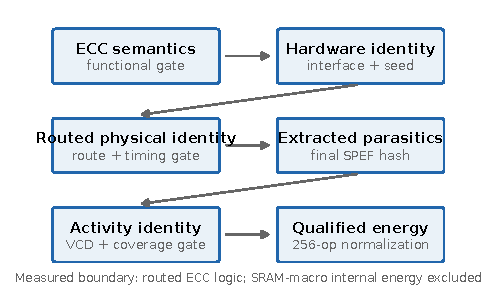
\includegraphics[width=\columnwidth]{figures/final/figure01_evidence_pipeline.pdf}
  \caption{Matched evidence pipeline. The architecture/seed identity used for timing is preserved through final-netlist activity and final-SPEF power analysis. The measured boundary is ECC logic, not SRAM-macro internals or a complete memory.}
  \label{fig:pipeline}
\end{figure}

This paper makes three contributions. First, it formulates energy ordering as an activity-conditional claim and evaluates it without changing the physical implementation between vectorless and activity-annotated analysis. Second, it contributes a fully paired dataset comprising ten timing-feasible physical runs, 46 qualified activity records, and 23 matched operation/seed comparisons. Third, it shows a concrete ranking failure: the diagnostic vectorless model favors Hsiao in 5/5 seeds, whereas operation-specific energy favors it in only 4/23 cells. The result is deliberately conditional, not universal: it demonstrates that architecture, physical state, and activity abstraction must be named together when reporting ECC energy.

\section{Related Work and Missing Comparison}
Hsiao's construction minimizes odd-weight parity-check columns for SECDED codes~\cite{hsiao1970}. Subsequent work targets ECC latency, protected-bit choices, or stronger correction, including low-delay data-bit protection~\cite{reviriego2013}, parallel double-error correction~\cite{naseer2008}, and SECDED/DAEC constructions~\cite{tripathi2020}. System and memory studies trade redundancy, coverage, storage density, and adaptation~\cite{delbel2014,pajouhi2015,wei2020,lee2022}. These works motivate architecture exploration but do not make an energy ranking independent of workload.

The closest power-focused work is Ghosh \emph{et al.}~\cite{ghosh2004}, which explicitly uses SPEC and MediaBench traces to restructure memory ECC checkers. That study establishes the relevance of real activity and prevents a broad claim that trace-driven ECC power analysis is new. Our narrower contribution differs along the controlled comparison: we hold each final routed implementation and its extracted parasitics fixed, apply both a vectorless diagnostic and explicit operation traces, and test whether the Hamming-versus-Hsiao ordering changes across the same five seeds. The object of study is therefore \emph{ordering validity under an activity-model substitution}, not a new ECC code or a new low-power checker transformation.

Open-source flows have made reproducible RTL-to-GDS studies practical~\cite{ajayi2019,shalan2020}, but flow reproducibility alone does not ensure evidence identity. A report can combine a timing number from one implementation state, activity from another netlist, or parasitics from a different seed. Equivalence checking addresses functional transformations~\cite{kuehlmann1997,kuehlmann2002}; our complementary concern is artifact lineage in downstream physical and power measurements. We therefore key every activity record by architecture, seed, final-netlist hash, SPEF hash, workload hash, and source-result hash.

\section{Experimental Method}
\subsection{Designs and controlled variables}
The evaluated designs implement the same memory-facing behavior and 64-bit data width with SECDED protection. The conventional implementation uses a Hamming-style parity-check organization; the comparison design uses Hsiao odd-weight columns. Both expose identical request, data, address, status, and clock/reset interfaces. Directed and randomized RTL checks cover clean access, single-bit correction, double-bit detection, and memory semantics before physical implementation. Functional equivalence between differently encoded internal representations is established at the interface rather than by requiring identical codewords.

All physical runs use the SKY130 high-density library at the nominal typical corner, a 10-ns clock target, and seeds 11, 13, 17, 19, and 23. Each architecture/seed pair is synthesized, placed, clock-tree synthesized, routed, and extracted by the same OpenROAD-based flow. A comparison enters the energy analysis only when routing succeeds and setup timing is feasible. We retain seed pairing instead of pooling unmatched runs because seed-specific placement and routing variation can be comparable to small architecture deltas.

\subsection{Question, estimand, and controls}
The tested null proposition is that changing only the activity abstraction leaves the direction of the architecture comparison unchanged. The vectorless observation for seed $s$ is the sign of $P^{V}_{\mathrm{Hsiao},s}-P^{V}_{\mathrm{conv.},s}$. The operation observation is the sign of $E^{A}_{\mathrm{Hsiao},s,o}-E^{A}_{\mathrm{conv.},s,o}$. Because power and energy have different units, we do not compare their magnitudes. We compare the induced binary ordering: which matched architecture is lower under each estimator. A failure occurs whenever the vectorless winner for a seed is not the activity-annotated winner for an available operation at that seed.

This design separates three forms of variation. \emph{Architectural variation} is the conventional-versus-Hsiao parity organization. \emph{Physical variation} is represented by the five seeds and controlled through within-seed pairing. \emph{Activity variation} is represented by the estimator and operation class while holding the routed circuit fixed. Table~\ref{tab:controls} makes the controlled and intentionally varying factors explicit. The distinction is important: an unpaired comparison could attribute a placement outlier to the code, while regenerating a netlist for each workload could attribute synthesis variation to activity.

\begin{table}[t]
\caption{Experimental controls and intentionally varied factors.}
\label{tab:controls}
\centering\footnotesize
\setlength{\tabcolsep}{3.2pt}
\begin{tabular}{p{0.27\columnwidth}p{0.63\columnwidth}}
\toprule
Factor & Treatment \\
\midrule
Varied & parity organization; seed; activity estimator; operation class \\
Held fixed & interface, 64-bit data, SECDED capability, 10-ns target, flow, PDK/library/corner, constraints \\
Paired by & physical seed and qualification state \\
Identity bound by & architecture, seed, netlist, SPEF, VCD/workload, and result hashes \\
Excluded & SRAM-internal and whole-memory energy; silicon measurement \\
\bottomrule
\end{tabular}
\end{table}

We use a sign-count estimand because it directly addresses whether a ranking survives. Means and sample standard deviations describe effect magnitude and seed dispersion but are secondary. With $n\leq5$ per operation, a parametric population model would add assumptions without resolving generality. The complete paired values are therefore the primary statistical object; no outlier rejection, seed weighting, or missing-value substitution is performed.

\subsection{Identity-preserving power protocol}
For each qualified run, simulation uses the exact final zero-delay routed gate netlist associated with the timing result. The resulting VCD is paired with that run's final SPEF. Hash equality, rather than only a shared filename stem, binds architecture, seed, netlist, parasitics, workload, and power result. This makes the experiment a substitution of activity assumptions on a fixed physical state.

We separate two estimators. The \emph{vectorless diagnostic} is the flow's default activity assumption and reports total logic power. The \emph{operation-specific estimator} annotates measured VCD activity for five classes: idle, clean write, clean read, correctable single-bit read, and detectable double-bit read. Sixteen warm-up cycles precede each measurement window, and every record contains 256 measured operations. Operation energy is
\begin{equation}
  E_{a,s,o}=P_{a,s,o}T_{s,o}/N_o,
\end{equation}
where $a$ is architecture, $s$ is physical seed, $o$ is operation class, $P$ is annotated ECC-logic power, $T$ is measured duration, and $N_o=256$. The paired comparison is
\begin{equation}
  \Delta E_{s,o}=E_{\mathrm{Hsiao},s,o}-E_{\mathrm{conv.},s,o}.
\end{equation}
Negative $\Delta E$ favors Hsiao. We report every pair and the arithmetic mean across available matched seeds; with only four or five pairs per operation, we avoid population-level significance claims.

\subsection{Activity completeness and qualification}
Every activity run covers all 72 SRAM-output activity roots. Functional logic coverage spans \CoverageMin--\CoverageMax\%, with 100\% sequential coverage and approximately 99.2\% combinational coverage. Coverage is a measurement-quality check, not evidence that the five synthetic operation classes represent an application's long-run distribution. Two seed-11 classes, idle and write, lack a qualified counterpart, leaving four pairs for those classes and five for each read-derived class. We do not impute missing values.

The 46 records arise as follows: both architectures contribute five seeds for clean read, correction, and detection (30 records), while idle and clean write each contribute four matched seed pairs (16 records). A record is admitted only after successful activity parsing, complete binding to the routed design, all 72 macro-output roots being represented, and successful power analysis. This accounting makes the denominator behind every sign count auditable. In particular, ``4/23'' is not a rounded percentage inferred from aggregate power; it is the count of negative paired $\Delta E$ values over all available cells.

There are two timing concepts in the protocol. Setup WNS qualifies whether the physical implementation can support the 10-ns target. Measurement duration normalizes annotated power to energy per completed operation. We do not convert WNS into a frequency-derived energy metric, and we do not compare raw average power across operation windows of different durations. This prevents timing headroom and window length from being conflated with the per-operation result.

The energy boundary includes synthesized and routed ECC logic at the memory interface. The SRAM macro is represented physically and functionally, but macro-internal switching energy is unavailable in the open characterization used here. Accordingly, all energy values and rankings are qualified as \emph{ECC-logic} results. They must not be read as whole-memory, chip, or silicon energy.

\section{Results}
\subsection{Physical qualification}
All ten 10-ns implementations route successfully and have nonnegative setup WNS. Across the five paired seeds, Hsiao minus conventional mean deltas are $+\AreaDelta~\mu\mathrm{m}^2$ total instance area, $+237.2~\mu\mathrm{m}^2$ standard-cell area, $+\WireDelta~\mu\mathrm{m}$ wirelength, $+\ViaDelta$ vias, and $+\WnsDelta$ ns setup WNS. Hsiao has better setup WNS in four of five pairs. These data reject a convenient explanation that activity results compare a feasible design with an infeasible one: both populations meet the chosen target.

\begin{figure*}[t]
  \centering
  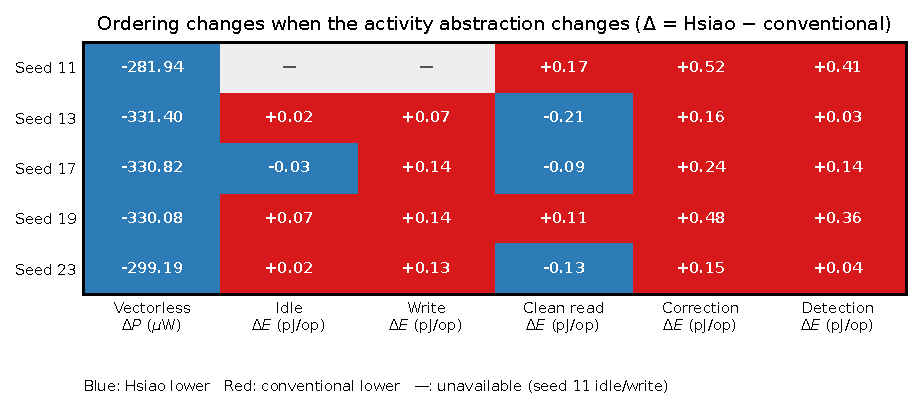
\includegraphics[width=0.94\textwidth]{figures/final/figure02_activity_ordering.pdf}
  \caption{Per-seed architecture ordering. Each cell reports Hsiao minus conventional. Vectorless cells use $\mu$W; operation cells use pJ/operation. Blue favors Hsiao and red favors conventional SECDED. The vectorless ordering is unanimous, but it is not preserved by operation-specific activity. Missing seed-11 idle/write pairs are shown rather than imputed.}
  \label{fig:ordering}
\end{figure*}

\subsection{The vectorless ordering does not survive}
Figure~\ref{fig:ordering} places the diagnostic and operation-specific comparisons side by side. Under vectorless estimation, Hsiao reports lower total logic power for all five seeds. Once operation activity is supplied, Hsiao is lower in only \ActivityHsiaoLower/\ActivityCells\ matched cells. The contrast is not produced by comparing different routed outcomes: each column's values derive from the same ten physical identities used for qualification.

Table~\ref{tab:headline} resolves the activity result by operation. Clean read is the only class with a negative mean Hsiao delta, $-0.0308$ pJ/op, and even there the sign is not unanimous (3/5). Conventional SECDED is lower in every available write pair, every correction pair, and every detection pair. Idle favors Hsiao in only 1/4 pairs. Thus neither the vectorless sign nor a single operation's mean is a reliable surrogate for all operations.

% Generated by scripts/build_artifacts.py
\begin{table}[t]
\caption{Operation-specific matched energy ordering at 10 ns. $\Delta E=E_{\mathrm{Hsiao}}-E_{\mathrm{conv.}}$.}
\label{tab:headline}
\centering\footnotesize
\setlength{\tabcolsep}{3.1pt}
\begin{tabular}{lrrrr}
\toprule
Operation & $n$ & Mean $\Delta E$ & Range & Hsiao lower \\
 & & (pJ/op) & (pJ/op) & \\
\midrule
Idle & 4 & +0.0191 & -0.029--+0.068 & 1/4 \\
Write & 4 & +0.1207 & +0.073--+0.139 & 0/4 \\
Clean read & 5 & -0.0308 & -0.213--+0.171 & 3/5 \\
Correction & 5 & +0.3095 & +0.148--+0.521 & 0/5 \\
Detection & 5 & +0.1935 & +0.030--+0.405 & 0/5 \\
\bottomrule
\end{tabular}
\end{table}


\subsection{Seed dispersion and operation dependence}
Figure~\ref{fig:deltas} exposes all 23 paired values rather than only aggregate bars. The Hsiao-minus-conventional mean deltas are $+0.0191$ pJ/op for idle, $+0.1207$ for write, $-0.0308$ for clean read, $+0.3095$ for correction, and $+0.1935$ for detection. Ranges and sample standard deviations in the generated result table show why five-seed pairing matters: clean-read deltas span $-0.213$ to $+0.171$ pJ/op, so a single seed could support either ordering.

\begin{figure}[t]
  \centering
  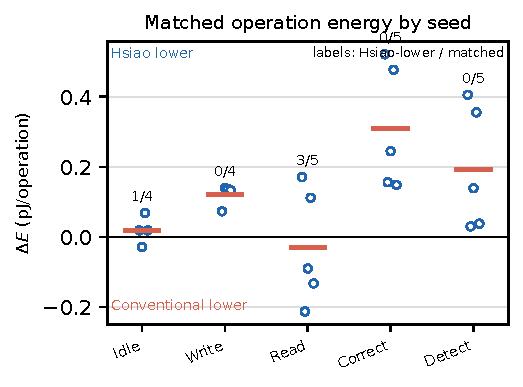
\includegraphics[width=\columnwidth]{figures/final/figure03_operation_energy_deltas.pdf}
  \caption{All matched operation-energy deltas; short orange bars are means and open circles are physical seeds. A zero reference separates Hsiao-lower (negative) from conventional-lower (positive) results. Counts above each operation give Hsiao-lower pairs over available pairs.}
  \label{fig:deltas}
\end{figure}

The component reports provide a mechanism-level check. On clean reads, Hsiao's switching component is lower in 5/5 seeds (mean $-28.97~\mu$W), while its internal component is higher in 5/5 (mean $+25.89~\mu$W); their competition produces the mixed total sign. For correction, the mean internal increase is $+35.46~\mu$W while the switching change is only $-4.52~\mu$W, yielding positive total deltas in every pair. Detection shows the same qualitative balance: $+30.42~\mu$W internal versus $-11.07~\mu$W switching. Write switching rises by $+12.18~\mu$W on average and all total deltas are positive. Leakage deltas are orders of magnitude smaller. These decompositions make the reversal physically interpretable: lower switching in selected cones does not guarantee lower total operation energy when internal power and exercised paths change.

\begin{figure}[t]
  \centering
  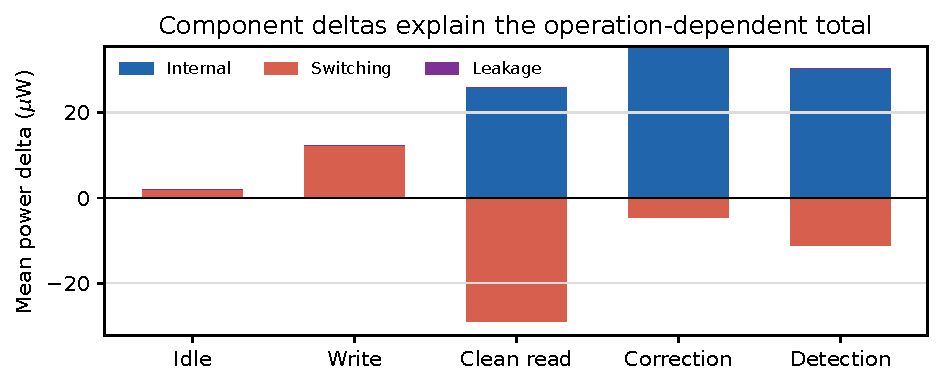
\includegraphics[width=\columnwidth]{figures/final/figure04_component_decomposition.pdf}
  \caption{Mean Hsiao-minus-conventional power-component deltas across available matched seeds. Internal and switching terms oppose one another for several read modes; leakage is visually negligible at this scale. Component means diagnose the total but do not replace the per-seed energy comparison.}
  \label{fig:components}
\end{figure}

Figure~\ref{fig:components} also cautions against using ``toggle reduction'' as a synonym for energy reduction. Clean read, correction, and detection all have negative mean switching deltas, yet only clean read has a negative mean total-energy delta. Library internal power responds to state-dependent charging within cells and can dominate a net-switching benefit. The specific component split is library- and tool-dependent, but the logical implication is general: parity-matrix weight alone does not determine the signed total after mapping, buffering, routing, and operation-specific sensitization.

\subsection{Answer to the research question}
For this matched implementation population, architecture energy ordering is \emph{not invariant} to the activity abstraction. The vectorless diagnostic's unanimous Hsiao-lower ordering fails for 19 of 23 operation-specific cells and for four of five operation means. The defensible claim is conditional: a vectorless ranking should not be promoted to an operation-energy ranking without retaining physical identity, applying relevant switching activity, and stating the measurement boundary.

\section{Discussion}
\subsection{Implications for ECC evaluation}
First, an ECC paper should report the tuple (architecture, implementation state, timing qualification, activity source, operation normalization, boundary), not only ``power.'' This tuple distinguishes a reproducible measurement from an architecture label. Second, workloads should be represented as mixtures of measured operations rather than by one default toggle rate. If $w_o$ is the fraction of operation $o$, a deployment-specific logic-energy difference is $\sum_o w_o\overline{\Delta E_o}$, subject to compatible idle accounting. Our data allow that calculation but do not prescribe $w_o$ for an application. Third, multiple seeds are not decorative replication. They reveal that the small clean-read advantage changes sign with physical realization even though correction, detection, and write results are stable over available pairs.

\subsection{Workload mixtures and crossover behavior}
The operation means support a transparent, limited ``what-if'' calculation. Ignoring idle and assuming active requests are partitioned among write ($w_W$), clean read ($w_R$), correction ($w_C$), and detection ($w_D$), with weights summing to one, the mean logic-energy delta is
\begin{equation}
 \overline{\Delta E}=0.1207w_W-0.0308w_R+0.3095w_C+0.1935w_D.
\end{equation}
For a clean-read/write-only workload, Hsiao has a negative mean only when the clean-read fraction exceeds approximately $0.797$. Even this crossover is illustrative rather than predictive because it uses unweighted seed means and excludes macro energy. Introducing rare error-handling events moves the mean toward conventional SECDED because both correction and detection deltas are positive in all five pairs. The equation is useful precisely because it states the workload assumption instead of hiding it inside a default activity factor.

Idle requires care. Its energy is normalized per scheduled idle operation window, not per wall-clock second of an unconstrained residency state. A system-level analysis should combine active operation energies with an explicitly defined idle-time model and the SRAM macro's standby behavior. Adding our idle mean directly to every request would double count time. We publish the underlying power and duration fields so another analysis can perform a compatible normalization.

The mixture analysis does not establish an optimal architecture. It demonstrates how qualified operation primitives can replace a single ranking with a workload-conditional decision surface. Such a surface can be combined with reliability rate, latency, and area constraints, but those objectives require explicit weights or Pareto analysis. The present experiment keeps them outside the central claim.

\subsection{A minimum reporting contract}
Our results suggest a compact reporting contract for pre-silicon ECC energy comparisons. Authors should state: (1) the exact logic and memory boundary; (2) whether power is vectorless, probabilistic, or waveform-annotated; (3) the netlist stage and timing model used to create activity; (4) the parasitic artifact and corner used for power; (5) operation definitions, warm-up, duration, and completed-operation count; (6) activity coverage; (7) physical qualification and seed pairing; and (8) every missing or rejected run. A digest-backed record is preferable when filenames can be overwritten.

This contract is intentionally independent of a particular commercial or open-source tool. A proprietary flow can preserve identity just as rigorously, and an open flow can lose it. The reproducibility contribution here is the linkage among artifacts and the explicit admission rule, not the mere availability of tool executables.

The finding does not argue that Hsiao codes are inefficient. Hsiao constructions remain attractive for their check-matrix properties, and different synthesis, pipeline, voltage, library, or workload choices may reverse our result. Nor does it argue that vectorless reports are useless: they remain valuable early diagnostics. The failure is treating the diagnostic ordering as a workload-independent design conclusion.

\subsection{Relationship to broader design tradeoffs}
ECC choice is only one axis. Stronger BCH-class correction introduces qualitatively different syndrome and search structures; low-power Chien-search architectures exist precisely because those costs require targeted treatment. Temporal transformations such as pipelining can trade latency and area for frequency or energy, while structural hierarchy can trade wire topology against logic depth. These axes are useful context, but mixing them into the present comparison would confound the activity question. We therefore keep code strength, interface, schedule, physical flow, and target period fixed and restrict the primary claim to conventional versus Hsiao SECDED.

\section{Threats to Validity}
\textbf{Workload representativeness.} The five operation classes are controlled micro-workloads, not traces from a specific processor or memory system. They establish that ordering can change and quantify the sampled classes; they do not estimate an application average. Application traces and operation weights are needed for deployment claims.

\textbf{Power-model scope.} Activity is captured from zero-delay simulation of the final routed netlist and combined with extracted parasitics. This preserves structure and exercised transitions but does not model delay-induced glitch activity with back-annotated timing. The reported numbers are tool/model estimates, not current measurements. Voltage, temperature, and library corner are fixed.

\textbf{Memory boundary.} SRAM-internal read, write, precharge, and leakage energy are excluded. This is the most important scope limitation: a macro model could dilute or amplify the ECC-logic delta. We therefore avoid whole-memory and sustainability claims.

\textbf{Population size and missing cells.} Five physical seeds support paired descriptive inference, not broad statistical generalization. Idle and write have four pairs because seed 11 lacks qualified records. No imputation is used. A larger seed set would narrow uncertainty around small means, especially clean read.

\textbf{Estimator dependence.} The vectorless settings form one diagnostic baseline, not the universe of probabilistic estimators. Another toggle-rate or correlation model might produce another ordering. That possibility reinforces, rather than weakens, the conditional conclusion, but it means our 5/5 vectorless observation should not be generalized to all vectorless configurations.

\textbf{Generality.} Results cover one data width, technology/library, target period, toolchain, constraint set, and two SECDED organizations. They establish non-invariance for the evaluated population rather than a universal ranking of Hamming and Hsiao logic. Replication at other nodes, frequencies, widths, and pipelines is future work.

\textbf{Functional and provenance assurance.} Interface-level tests and activity coverage reduce, but do not eliminate, functional-validation risk. Hashes establish artifact identity, not semantic correctness. Independent reruns and formal cross-architecture property checks would strengthen assurance.

\textbf{Researcher degrees of freedom.} The central question, delta direction, five operation classes, seed set, timing gate, and no-imputation rule are fixed by the sealed campaign artifacts. We report sign counts and full cells to limit selective aggregation. The study was not preregistered, so confirmation on a separately generated seed population remains valuable.

\balance
\section{Replication and Falsification Protocol}
The result can be independently challenged at three levels. A \emph{numerical audit} begins from the 46 admitted activity records and recomputes each operation energy, pairs equal seeds, and evaluates $\Delta E$ with the declared direction. It should recover 23 cells, four negative deltas, and the means in Table~\ref{tab:headline}. It should also find no seed-11 idle or write pair. This level tests aggregation, units, and missing-data handling without rerunning implementation tools.

An \emph{artifact audit} additionally verifies that each record's final-netlist and SPEF digests match the architecture and seed that supplied timing qualification, that all records name the operation workload digest, and that the VCD binds to the routed netlist. It then checks the activity admission rule: 16 warm-up cycles, 256 measured operations, all 72 macro-output roots, and the stated coverage range. This level can falsify the identity-preservation premise even if the arithmetic is correct. A mismatched SPEF, a pre-route netlist, or an incomplete root set invalidates the affected cell rather than merely widening its uncertainty.

A \emph{flow replication} regenerates physical and activity artifacts from RTL under the declared toolchain. Exact numeric equality is not expected across tool or library revisions, so the replication should record its own versions and digests. The relevant outcomes are: physical feasibility at 10 ns, the vectorless per-seed sign, the operation-specific per-seed signs, and component decomposition. Additional seeds should be reported as a new population, not silently merged with the sealed five. A replication that preserves the controls but obtains the same winner for every vectorless and activity cell would falsify the observed non-invariance for that new population; one that changes only under some operations would extend it.

The package supporting this protocol retains four representations of each used figure: the plotting script, source CSV or JSON, vector PDF/SVG, and high-resolution PNG. Derived tables are generated from the same machine-readable rows. The reproducibility ledger carries architecture, seed, target period, technology/library/corner, route and timing state, netlist/SPEF/VCD/workload digests, coverage, window definition, power components, energy, qualification, and source-result digest. Candidate and analysis plots are retained with their dispositions so page-limit decisions cannot erase contrary or diagnostic views.

Three extensions would most strengthen the conclusion. First, sample a preregistered second seed set and report paired intervals without reselecting operations. Second, replay application traces and publish the operation mixture used to create any aggregate; this connects our controlled primitives to use cases while respecting prior trace-driven ECC work~\cite{ghosh2004}. Third, add characterized macro read, write, and standby energy with a clearly separable boundary. That experiment would determine whether the logic-level ordering survives once the dominant memory-array terms are included. Until then, the correct object is ECC-logic energy, and any whole-memory inference remains explicitly untested.

\section{Conclusion}
We asked whether an ECC energy ordering remains valid when vectorless activity is replaced by operation-specific switching while physical qualification and parasitic identity are preserved. In ten timing-feasible post-route implementations, vectorless reports favored Hsiao SECDED in 5/5 matched seeds. Final-netlist activity with final parasitics favored Hsiao in only 4/23 matched operation/seed cells; conventional SECDED was lower for every available write, correction, and detection pair. The reversal is explained by operation-dependent competition between switching and internal power and by seed-level physical variation. The result is not a universal preference for one code. It is a measurement rule: ECC energy ordering is conditional on activity, implementation state, normalization, and boundary. Claims that omit those qualifiers can invert when evaluated on the operations the circuit actually performs.

\clearpage
\balance
\bibliographystyle{IEEEtran}
\bibliography{references}
\end{document}
